\documentclass[a4paper,onecolumn,oneside,12pt,extrafontsizes]{memoir}
\usepackage[utf8]{inputenc}
\usepackage[T1]{fontenc}
\usepackage[english,polish]{babel}
\usepackage{setspace}
\usepackage{color,calc}
\usepackage{ebgaramond}
\usepackage{tgtermes}
\usepackage{float}
\usepackage{silence}

\renewcommand*\ttdefault{txtt}

\clubpenalty=10000
\widowpenalty=10000
\righthyphenmin=3

\renewcommand{\topfraction}{0.95}
\renewcommand{\bottomfraction}{0.95}
\renewcommand{\textfraction}{0.05}
\renewcommand{\floatpagefraction}{0.35}

\setlength{\headsep}{10pt}
\setlength{\headheight}{13.6pt}
\setlength{\footskip}{\headsep+\headheight}
\setlength{\uppermargin}{\headheight+\headsep+1cm}
\setlength{\textheight}{\paperheight-\uppermargin-\footskip-1.5cm}
\setlength{\textwidth}{\paperwidth-5cm}
\setlength{\spinemargin}{2.5cm}
\setlength{\foremargin}{2.5cm}
\setlength{\marginparsep}{2mm}
\setlength{\marginparwidth}{2.3mm}

\checkandfixthelayout[fixed]

\linespread{1}
\setlength{\parindent}{14.5pt}

\usepackage{multicol}
\usepackage{tabularx}
\usepackage{listings}
\usepackage{xpatch}
\makeatletter
\xpatchcmd\l@lstlisting{1.5em}{0em}{}{}
\makeatother

\lstset{
  basicstyle=\small\ttfamily,
  breaklines=true,
  postbreak=\mbox{\textcolor{red}{$\hookrightarrow$}\space},
  belowskip=.5\baselineskip,
  literate={\_}{{\_\allowbreak}}1,
  extendedchars=true,
  inputencoding=utf8,
  keepspaces=true
}

\definecolor{lightgray}{rgb}{.9,.9,.9}
\definecolor{darkgray}{rgb}{.4,.4,.4}
\definecolor{purple}{rgb}{0.65, 0.12, 0.82}
\definecolor{javared}{rgb}{0.6,0,0} % for strings
\definecolor{javagreen}{rgb}{0.25,0.5,0.35} % comments
\definecolor{javapurple}{rgb}{0.5,0,0.35} % keywords
\definecolor{javadocblue}{rgb}{0.25,0.35,0.75} % javadoc
\definecolor{codegreen}{rgb}{0.125,0.5,0.25}
\definecolor{codeblue}{rgb}{0.125,0.25,0.75}
\definecolor{codegray}{rgb}{0.5,0.5,0.5}
\definecolor{backcolour}{rgb}{0.95,0.95,0.95}

% Definicja języka JavaScript
\lstdefinelanguage{JavaScript}{
    keywords={typeof, new, true, false, catch, function, return, null, catch, switch, var, if, in, while, else, case, break, export, default, import, let, const, async, await, type},
    keywordstyle=\color{codeblue}\bfseries,
    ndkeywords={class, export, boolean, throw, implements, import, this, useState, default},
    ndkeywordstyle=\color{codegreen}\bfseries,
    identifierstyle=\color{black},
    sensitive=false,
    comment=[l]{//},
    morecomment=[s]{/*}{*/},
    commentstyle=\color{codegreen}\ttfamily,
    stringstyle=\color{codegreen}\ttfamily,
    morestring=[b]',
    morestring=[b]"
}

\definecolor{pblue}{rgb}{0.13,0.13,1}
\definecolor{pgreen}{rgb}{0,0.5,0}
\definecolor{pred}{rgb}{0.9,0,0}
\definecolor{pgrey}{rgb}{0.46,0.45,0.48}
\definecolor{dark-grey}{rgb}{0.4,0.4,0.4}

\newcommand\JSONnumbervaluestyle{\color{blue}}
\newcommand\JSONstringvaluestyle{\color{red}}

\newif\ifcolonfoundonthisline

\makeatletter

\lstdefinestyle{json-style}
{
	showstringspaces    = false,
	keywords            = {false,true},
	alsoletter          = 0123456789.,
	morestring          = [s]{"}{"},
	stringstyle         = \ifcolonfoundonthisline\JSONstringvaluestyle\fi,
	MoreSelectCharTable =%
	\lst@DefSaveDef{`:}\colon@json{\processColon@json},
	basicstyle          = \footnotesize\ttfamily,
	keywordstyle        = \ttfamily\bfseries,
	numbers				= left,
	numberstyle={\footnotesize\ttfamily\color{dark-grey}},
	xleftmargin			= 2em
}

\newcommand\processColon@json{
	\colon@json
	\ifnum\lst@mode=\lst@Pmode
	\global\colonfoundonthislinetrue
	\fi
}

\lst@AddToHook{Output}{
	\ifcolonfoundonthisline
	\ifnum\lst@mode=\lst@Pmode
	\def\lst@thestyle{\JSONnumbervaluestyle}
	\fi
	\fi
	\lsthk@DetectKeywords
}

\lst@AddToHook{EOL}
{\global\colonfoundonthislinefalse}

\makeatother

\usepackage{memlays}
\usepackage{printlen}
\usepackage{enumitem}

\uselengthunit{pt}
\makeatletter
\newcommand{\showFontSize}{\f@size pt} % makro wypisujące wielkość bieżącej czcionki
\makeatother

\usepackage{enumitem}
\setlist{noitemsep,topsep=4pt,parsep=0pt,partopsep=4pt,leftmargin=*}
\setenumerate{labelindent=0pt,itemindent=0pt,leftmargin=!,label=\arabic*.}
\setlistdepth{4}
\setlist[itemize,1]{label=$\bullet$}
\setlist[itemize,2]{label=\normalfont\bfseries\textendash}
\setlist[itemize,3]{label=$\ast$}
\setlist[itemize,4]{label=$\cdot$}
\renewlist{itemize}{itemize}{4}

\makeatletter
\renewenvironment{quote}{
	\begin{list}{}
	{
	\setlength{\leftmargin}{1em}
	\setlength{\topsep}{0pt}%
	\setlength{\partopsep}{0pt}%
	\setlength{\parskip}{0pt}%
	\setlength{\parsep}{0pt}%
	\setlength{\itemsep}{0pt}
	}
	}{
	\end{list}}
\makeatother

\usepackage[pdftex,bookmarks,breaklinks,unicode]{hyperref}
\usepackage{hyperxmp}
\usepackage{ifpdf}

\ifpdf
 \usepackage{datetime2}
 \usepackage[pdftex]{graphicx}
 \DeclareGraphicsExtensions{.pdf,.jpg,.mps,.png}
\pdfcompresslevel=9
\pdfoutput=1

\makeatletter
\AtBeginDocument{
  \hypersetup{
	pdfinfo={
    Title = {\@title},
    Author = {\@author},
    Subject={Praca dyplomowa \ifMaster magisterska\else inżynierska\fi},
    Keywords={\@kvpl},
		Producer={},
	  CreationDate= {},
    ModDate={\pdfcreationdate},
		Creator={pdftex},
	}}
}

\pdftrailerid{}
\pdfsuppressptexinfo15
\makeatother
\else
\usepackage{graphicx}
\DeclareGraphicsExtensions{.eps,.ps,.jpg,.mps,.png}
\fi
\sloppy

\def\UrlBreaks{\do\/\do-\do_}

\setcounter{secnumdepth}{2}
\setcounter{tocdepth}{2}
\setsecnumdepth{subsection}

\makeatletter
\def\@seccntformat#1{\csname the#1\endcsname.\quad}
\def\numberline#1{\hb@xt@\@tempdima{#1\if&#1&\else.\fi\hfil}}
\makeatother

\renewcommand{\chapternumberline}[1]{#1.\quad}
\renewcommand{\cftchapterdotsep}{\cftdotsep}

\makeatletter
\renewcommand*{\insertchapterspace}{%
  \addtocontents{lof}{\protect\addvspace{3pt}}%
  \addtocontents{lot}{\protect\addvspace{3pt}}%
	\addtocontents{toc}{\protect\addvspace{3pt}} %
  \addtocontents{lol}{\protect\addvspace{3pt}}}
\makeatother

\setlength{\cftbeforechapterskip}{0pt}
\renewcommand{\aftertoctitle}{\afterchaptertitle\vspace{-4pt}}

\captionnamefont{\small}
\captiontitlefont{\small}

\newcommand{\listingcaption}[1]
{%
\vspace*{\abovecaptionskip}\small
\refstepcounter{lstlisting}\hfill%
Listing \thelstlisting: #1\hfill%\hfill%
\addcontentsline{lol}{lstlisting}{\protect\numberline{\thelstlisting}#1}
}%

\newcommand{\eng}[1]{(ang.~\emph{#1})}
\newcommand*{\captionsource}[2]{
  \caption[{#1}]{
    #1 \emph{Źródło:} #2
  }%
}

\addto\captionspolish{
\renewcommand{\tablename}{Tab.}
}

\addto\captionspolish{
\renewcommand{\figurename}{Rys.}
}

\addto\captionspolish{
\renewcommand{\lstlistlistingname}{Spis listingów}
}

\addto\captionspolish{
\renewcommand{\bibname}{Literatura}
}

\addto\captionspolish{
\renewcommand{\listfigurename}{Spis rysunków}
}

\addto\captionspolish{
\renewcommand{\listtablename}{Spis tabel}
}

\addto\captionspolish{
\renewcommand\indexname{Indeks rzeczowy}
}

\renewcommand{\abstractnamefont}{\normalfont\Large\bfseries}
\renewcommand{\abstracttextfont}{\normalfont}

\addtopsmarks{headings}{
    \nouppercaseheads
}{
\createmark{chapter}{both}{shownumber}{}{. \space}
\createmark{section}{right}{shownumber}{}{. \space}
}

\makeatletter
\copypagestyle{outer}{headings}
\makeoddhead{outer}{}{}{\small\itshape\rightmark}
\makeevenhead{outer}{\small\itshape\leftmark}{}{}
\makeoddfoot{outer}{\small\@author:~\@titleShort}{}{\small\thepage}
\makeevenfoot{outer}{\small\thepage}{}{\small\@author:~\@title}
\makeheadrule{outer}{\linewidth}{\normalrulethickness}
\makefootrule{outer}{\linewidth}{\normalrulethickness}{2pt}
\makeatother

\copypagestyle{plain}{headings}
\makeoddhead{plain}{}{}{}
\makeevenhead{plain}{}{}{}
\makeevenfoot{plain}{}{}{}
\makeoddfoot{plain}{}{}{}

\copypagestyle{empty}{headings}
\makeoddhead{empty}{}{}{}
\makeevenhead{empty}{}{}{}
\makeevenfoot{empty}{}{}{}
\makeoddfoot{empty}{}{}{}

\newif\ifMaster

\makeatletter
%Uczelnia
\newcommand\uczelnia[1]{\renewcommand\@uczelnia{#1}}
\newcommand\@uczelnia{}
%Wydział
\newcommand\wydzial[1]{\renewcommand\@wydzial{#1}}
\newcommand\@wydzial{}
%Kierunek
\newcommand\kierunek[1]{\renewcommand\@kierunek{#1}}
\newcommand\@kierunek{}
%Specjalność
\newcommand\specjalnosc[1]{\renewcommand\@specjalnosc{#1}}
\newcommand\@specjalnosc{}
%Tytuł po angielsku
\newcommand\titleEN[1]{\renewcommand\@titleEN{#1}}
\newcommand\@titleEN{}
%Tytuł krótki
\newcommand\titleShort[1]{\renewcommand\@titleShort{#1}}
\newcommand\@titleShort{}
%Promotor
\newcommand\promotor[1]{\renewcommand\@promotor{#1}}
\newcommand\@promotor{}
%Słowa kluczowe
\newcommand\kvpl[1]{\renewcommand\@kvpl{#1}}
\newcommand\@kvpl{}
\newcommand\kven[1]{\renewcommand\@kven{#1}}
\newcommand\@kven{}
%Komenda wykorzystywana w streszczeniu
\newcommand\mykeywords{\hspace{\absleftindent}%
\parbox{\linewidth-2.0\absleftindent}{
       \iflanguage{polish}{\textbf{Słowa kluczowe:} \@kvpl}{%
			 \iflanguage{english}{\textbf{Keywords:} \@kven}}{}}
				}

\def\maketitle{
  \pagestyle{empty}
    \fontfamily{\ebgaramond@family}\selectfont

\newlength{\tmpfboxrule}
\setlength{\tmpfboxrule}{\fboxrule}
\setlength{\fboxsep}{2mm}
\setlength{\fboxrule}{0mm}

\setlength{\unitlength}{1mm}
\begin{picture}(0,0)

\put(20,-124){\fbox{
\parbox[c][71mm][c]{104mm}{\centering
{\fontsize{18pt}{20pt}\bfseries\selectfont \@title}\\[5mm]
{\fontsize{18pt}{20pt}\bfseries\selectfont \@titleEN}\\[10mm]
{\fontsize{16pt}{18pt}\selectfont \@author}}
}
}
\end{picture}
\setlength{\fboxrule}{\tmpfboxrule}
{\vskip 9pt\centering
		{\fontsize{20pt}{22pt}\bfseries\selectfont \@uczelnia}\\[5pt]
		{\fontsize{16pt}{18pt}\bfseries\selectfont \@wydzial}\\[1pt]
		  \hrule
	}
{\vskip 24pt\raggedright\fontsize{14pt}{16pt}\selectfont%
\begin{tabular}{@{}ll}
Kierunek: & {\bfseries \@kierunek}\\
Specjalność: & {\bfseries \@specjalnosc}\\
\end{tabular}\\[1.3cm]
}
{\vskip 29pt\centering{\fontsize{24pt}{26pt}\selectfont%
{\fontsize{26pt}{28pt}\selectfont P}RACA {\fontsize{26pt}{24pt}\selectfont D}YPLOMOWA\\[7pt]
\ifMaster \selectfont{\fontsize{26pt}{28pt}\selectfont M}AGISTERSKA\\[2.5cm]%
\else \selectfont{\fontsize{26pt}{28pt}\selectfont I}NŻYNIERSKA\\[2.5cm]\fi
}}
	\vfill
{\centering
    {\fontsize{14pt}{16pt}\selectfont Opiekun pracy}\\[2mm]
	{\fontsize{14pt}{16pt}\bfseries\selectfont \@promotor}\\[10mm]
}
\vspace{4cm}\noindent
{\fontsize{12pt}{14pt}\selectfont Słowa kluczowe: \@kvpl}
\vspace{1.3cm}
\hrule\vspace*{0.3cm}
{\centering
{\fontsize{14pt}{16pt}\selectfont \@date}\\[0cm]
}
\normalfont
 \cleardoublepage
}
\makeatother

\title{Aplikacja webowa do optymalizacji zleceń w transporcie towarów} % INFO: tytuł pracy w języku polskim
\titleShort{Aplikacja webowa do optymalizacji zleceń w transporcie towarów}  % INFO: krótki tytuł pracy (do zamieszczenia w stopce, sklejony z imieniem i nazwiskiem autora nie powinien zająć więcej niż jedną linijkę)
\titleEN{Web application for optimizing orders in the transport of goods} % INFO: tytuł pracy w języku angielskim
\author{Krystian Tomczyk}  % INFO: imię i nazwisko autora
\uczelnia{Politechnika Wrocławska} % INFO: nazwa uczelni
\wydzial{Wydział Informatyki i Telekomunikacji} % INFO: nazwa wydziału
\kierunek{Informatyka techniczna (ITE)} % IFO: nazwa kierunku
\specjalnosc{Inżynieria systemów informatycznych (INS)} % INFO: nazwa specjalności
\promotor{dr. inż. Paweł Rogaliński} % INFO: dane promotora
\kvpl{aplikacja, transport, web} % INFO: słowa kluczowe po polsku
\kven{application, transport, web} % INFO: słowa kluczowe po angielsku
\date{WROCŁAW, 2025} % INFO: miejscowość, rok złożenia pracy dyplomowej

\begin{document}

\pdfbookmark[0]{Tytuł}{Tytul.1}
\maketitle

\pdfbookmark[0]{Streszczenie}{streszczenie.1}
\begin{abstract}
Niniejsza praca inżynierska dotyczy projektu aplikacji webowej CargoLink, zaprojektowanej w celu optymalizacji procesów logistycznych w transporcie towarów. Głównym celem systemu jest łączenie zleceniodawców i przewoźników, minimalizowanie pustych przebiegów oraz redukcja kosztów transportu. Aplikacja oferuje funkcje takie jak: dodawanie zleceń transportowych, publikowanie ogłoszeń o planowanych trasach, rekomendacje dopasowanych ofert oraz komunikację użytkowników poprzez wbudowany czat. System wspiera generowanie szablonów umów oraz umożliwia ocenę użytkowników po zakończeniu współpracy.

Pod względem technicznym aplikacja wykorzystuje nowoczesne technologie, takie jak TypeScript, Next.js, Tailwind CSS i PostgreSQL, zapewniające wysoką wydajność i bezpieczeństwo. W bazie danych zastosowano UUID jako klucze główne oraz algorytm bcrypt do szyfrowania haseł. Interfejs użytkownika zaprojektowano w programie Figma z uwzględnieniem responsywności oraz intuicyjnej obsługi.

Dokumentacja opisuje szczegółowo przypadki użycia systemu dla różnych aktorów oraz architekturę warstwową aplikacji. Przedstawiono również proces testowania systemu, w tym testy jednostkowe, end-to-end oraz wydajnościowe. Na zakończenie wskazano potencjalne kierunki rozwoju projektu, takie jak wprowadzenie nowych funkcjonalności i zwiększenie skalowalności systemu.
\end{abstract}
\mykeywords
{
\selectlanguage{english}
\begin{abstract}
This engineering thesis concerns the design of CargoLink web application, developed to optimize logistics processes in cargo transportation. The main goal of the system is to connect shippers with carriers, minimize empty runs, and reduce transportation costs. The application offers features such as: adding transport orders, publishing announcements about planned routes, recommending matched offers, and enabling user communication through a built-in chat. The system supports generating contract templates and allows users to rate each other after completed cooperation.

From a technical perspective, the application utilizes modern technologies such as TypeScript, Next.js, Tailwind CSS, and PostgreSQL, ensuring high performance and security. The database implements UUID as primary keys and uses the bcrypt algorithm for password encryption. The user interface was designed in Figma with consideration for responsiveness and intuitive operation.

The documentation thoroughly describes use cases for various actors and the layered architecture of the application. The system testing process is also presented, including unit tests, end-to-end tests, and performance tests. Finally, potential directions for project development are indicated, such as introducing new functionalities and increasing system scalability.
\end{abstract}
\mykeywords
}

\pagestyle{outer}
\clearpage

\pdfbookmark[0]{Spis treści}{spisTresci.1}
\tableofcontents*
\clearpage

\pdfbookmark[0]{Spis rysunków}{spisRysunkow.1}
\listoffigures*
\clearpage

% \pdfbookmark[0]{Spis tabel}{spisTabel.1}
% \listoftables*
% \clearpage

\pdfbookmark[0]{Spis listingów}{spisListingow.1}
\lstlistoflistings*
\clearpage

\chapterstyle{default}
\chapter{Wstęp}

Transport towarów odgrywa kluczową rolę w globalnej gospodarce, łącząc producentów i konsumentów na całym świecie. Efektywność transportu ma bezpośredni wpływ na koszty operacyjne firm oraz na ceny finalnych produktów \cite{MurphyWoodLogistyka}. W zależności od specyfiki przewożonych towarów oraz potrzeb zleceniodawców, transport może przyjmować dwie następujące formy:

\label{sec:przewoz_regularny}
Transport regularny, inaczej łańcuch dostaw, to przewóz towarów, który odbywa się według ustalonego harmonogramu i stałych tras. Charakteryzuje się regularnością kursów, co oznacza, że pojazdy wykonują swoje trasy w określonych, z góry ustalonych terminach. Przykładami transportu regularnego są linie autobusowe, kolejowe czy lotnicze, które działają według stałego rozkładu jazdy.

\label{sec:transport_okazjonalny}
Transport okazjonalny to przewóz towarów, który odbywa się bez ustalonego z góry rozkładu jazdy. Pojazdy wykonują swoje trasy w zależności od zapotrzebowania klientów, najczęściej jest to usługa jednorazowa. Sam przewóz zaś zlecany jest na potrzebę klienta, nie musi on jednak określać dokładnego terminu odbycia trasy, ani przez kogo ma on być zrealizowany.

Podczas swoich tras przewoźnicy czasami są zmuszeni do przebycia części drogi bez żadnego ładunku. Powoduje to, że przewozy nie są w pełni zoptymalizowane względem kosztów, jakie niesie za sobą pokonywana trasa. Możliwe jest jednak zredukowanie występowania takich sytuacji poprzez odpowiednie powiązanie przewoźników i osób zlecających transport okazjonalny. Zleceniodawca, który nie potrzebuje dostawy towaru w konkretnej dacie, mógłby wtedy zlecić transport z nieokreślonym dokładnie terminem dotarcia towaru, w zamian za niższe ceny przewozowe. Przykład: dyrektor szkoły, w czasie wakacji, zamówił dużych rozmiarów tablicę interaktywną, która nie zmieściłaby się w standardowym samochodzie osobowym. Z racji, że zamówienie zostało złożone w czasie, gdy dzieci nie chodzą do szkoły, nie zależy mu na dokładnym terminie dostawy. Może on w takim przypadku zlecić dostawę tablicy w formie transportu okazjonalnego, z mniejszymi kosztami transportu. Przewoźnik mógłby zabrać towar i zawieźć go na miejsce docelowe, gdy akurat wykonywałby trasę bez ładunku i kierował się w przybliżonym kierunku. Taka sytuacja jest korzystna dla obu stron, przewoźnik może odbywać przewozy bardziej efektywnie, dzięki nie marnowaniu zasobów na puste przebiegi. Zleceniodawca natomiast, może oczekiwać niższych kosztów przewozu towarów.

Połączenie między osobami zlecającymi usługi transportowe - zleceniodawcami, a osobami oferującymi przewóz towaru - przewoźnikami, może odbywać się za pomocą serwisu oferującego dodawanie publicznych ogłoszeń. Ogłoszenia dzielić się będą na dwie kategorie, ogłoszenie z planowaną trasą przejazdu oraz zlecenie z wymaganym towarem do przewiezienia z punktu początkowego do punktu docelowego.

\section{Cel i zakres projektu}
\label{sec:cele}
Celem projektu jest stworzenie aplikacji webowej, pod tytułem \texttt{CargoLink}. Serwis ten pozwalać będzie na dodawanie ogłoszeń oraz zleceń dotyczących transportów okazjonalnych. Aplikacja przyczni się do zoptymalizowania procesów logistycznych, eliminując nieefektywne wykorzystanie zasobów transportowych. Dodatkowo pozwoli ona przewoźnikom i zleceniodawcom, na łatwą i szybką komunikacje między sobą.
Główne cele projektu:
\begin{enumerate}
    \item \textbf{Możliwość umieszczania ogłoszeń i zleceń}: aplikacja pozwalać ma na dodawanie ogłoszeń o trasach przejazdu, planowanych przez przewoźników oraz zleceń transportowych na konkretny towar przez zleceniodawców
    \item \textbf{Ułatwienie szukania odpowiednich ogłoszeń i zleceń}: poprzez system powiązania zleceń transportowych do planowanych tras przewoźników oraz ogłoszeń o planowanej trasie do zleceń zamieszczonych w serwisie, aplikacja skróci czas potrzebny na znalezienie odpowiednich ofert.
    \item \textbf{Komunikacja między przewoźnikami i zleceniodawcami}: aplikacja umożliwi szybką komunikację między użytkownikami serwisu poprzez czat tekstowy.
    \item \textbf{Redukcja kosztów transportu}: dzięki lepszemu dopasowaniu potencjalnych przewoźników i zleceniodawców, aplikacja pozwoli na obniżenie kosztów transportu zarówno dla zleceniodawców, jak i przewoźników.
\end{enumerate}
Nowoczesna aplikacja transportowa powinna przyczynić się do efektywnego zrealizowania tych celów, co wspomoże rynek zleceń transportowych, przynosząc korzyści zarówno dla zleceniodawców, jak i przewoźników.

\section{Wymagania aplikacji}
Na podstawie analizy celów wymienionych w podrozdziale \ref{sec:cele}, można wywnioskować, że do efektywnego działania serwisu, będą musiały zostać zrealizowane następujące wymagania funkcjonalne:
\begin{enumerate}
    \item \textbf{Uwierzytelnianie}: aplikacja będzie wykorzystywała system rejestracji oraz logowania.
    \item \textbf{Regulanim}: podczas rejestrowania się do serwisu, użytkownik musi zaakceptować regulamin korzystania z aplikacji.
    \item \textbf{Dodawanie zleceń transportowych}: serwis pomagał będzie znaleźć odpowiedniego przewoźnika poprzez udostępnienie możliwości dodania ogłoszenia zlecenia. W ogłoszeniu zlecenia znajdować się będzie:
    \begin{itemize}
        \item tytułu zlecenia,
        \item opis zlecenia (niewymagane),
        \item wymagana trasa przewozu (miejsce startu oraz miejsce docelowe),
        \item przybliżony termin dostarczenia (przedział dat),
        \item waga towarów do przewiezenia,
        \item wymiary przewożonych dóbr,
        \item kategoria każdego z towarów,
        \item informacja o wymaganych specjalnych warunkach podczas transportu (np. jedzenie wymagać będzie przewozu w odpowiedniej temperaturze, pole niewymagane),
        \item imienia i nazwiska zleceniodawcy bądź nazwy firmy, która zleceniodawca reprezentuje,
    \end{itemize}
    \item \textbf{Dodawanie ogłoszeń o planowanej trasie}: system powinien pozwalać przewoźnikom, na dodawanie publicznych informacji o planowanych przez siebie trasach. Ogłoszenie będzie składało się z:
    \begin{itemize}
        \item tytułu ogłoszenia,
        \item opisu ogłoszenia (niewymagane),
        \item planowanej trasy przewozu (miejsce startu oraz miejsce docelowe),
        \item daty planowanego przejazdu,
        \item dostępnego miejsca w pojeździe (wymiary liczone w europaletach),
        \item maksymalnej wagi towaru,
        \item marki i modelu pojazdu,
        \item danych kontaktowych,
        \item imienia i nazwiska przewoźnika bądź nazwy firmy, która przewoźnik reprezentuje,
    \end{itemize}
    \item \textbf{System rekomendacji ogłoszeń}: podczas wprowadzania danych o trasie, użytkownik będzie informowany o sugerowanych zleceniach dodanych przez innych użytkowników (np. gdy zlecenie dotyczy trasy, która w przybliżeniu pokrywa się z tą jaką przewoźnik planuje się poruszać). Analogicznie gdy zleceniodawca zamierza dodać ogłoszenie zlecenia, zostanie on poimformowany o proponowanych ogłoszeniach przewoźników.
    \item \textbf{Umożliwienie konaktu między użytkownikami}: aby zapewnnić kontakt między użytkownikami, w aplikacji zostanie dodany czat tekstowy umożliwiający korespondencje między zleceniodawcami, a przewoźnikami, bezpośrednio w aplikacji. Ma on pełnić rolę komunikacji na wzór tej  oferowanej przez tradycyjną poczte elektroniczną.
    \item \textbf{Generowanie szablonu umowy}: przewoźnik i zleceniodawca, po negocjacji warunków umowy, otrzymają wygenerowany przez serwis szablon dokumentu finalizujący transakcje.
    \item \textbf{Weryfikacja dodawanych ogłoszeń}: zanim ogłoszenie wyświetlać się będzie dla wszystkich użytkowników, moderator serwisu będzię musiał je zatwierdzić.
    \item \textbf{Graficzne przedstawienie trasy}: podczas dodawania ogłoszenia o planowanej trasie, przewoźnikowi wyświetlać się będzie mapa z zaznaczonymi trasami, dodanymi przez zleceniodawców, które przebiegają w przybliżonym kierunku. Zleceniodawcy natomiast, podczas dodawania oferty, będą widzieć mapę ze wszystkimi trasami planowanymi przez przewoźników.
    \item \textbf{System ocen użytkownika}: po 2 dniach po upływie terminu przewozu, użytkownicy będą mogli dodać opinie na temat użytkownika, którego umowa dotyczyła. Opinia składała się będzie z oceny w skali 1-5 oraz komentarza. Opinie będą wyświetlały się na stronie porfilu tego użytkownika oraz na dodanych przez niego ogłoszeniach.
\end{enumerate}
Aplikacja musi być niezawodna i przyjazna do użytkowania dla wszystkich. Do komfortowego korzystania z serwisu przez użytkowników, niezbędna będzie realizacja następujących wymagań niefunkcjonalnych
\begin{enumerate}
    \item \textbf{Innowacyjność}: Aplikacja musi używać nowoczesnych technologii, takich jak \texttt{TypeScript}, \texttt{Next.js}, \texttt{Tailwind CSS}, \texttt{Node.js} oraz bazę danych \texttt{PostgreSQL}, zapewni to wysoką wydajność, skalowalność i bezpieczeństwo aplikacji.
    \item \textbf{Intuicyjny interfejs użytkownika}: Aplikacja musi posiadać prosty i intuicyjny interfejs użytkownika, który umożliwi łatwą obsługę zarówno dla zleceniodawców, jak i przewoźników.
    \item \textbf{Dostępność na różnych urządzeniach}: Aplikacja musi responsywna i dostosowana do różnych urządzeń, takich jak komputery, tablety i smartfony, co zapewni wygodę użytkowania w dowolnym miejscu i czasie.
    \item \textbf{Wielojęzyczność}: użytkownicy korzystający z aplikacji, muszą mieć możliwość wyboru jednego z trzech przewidzianych języków: polski, angielski oraz niemiecki. Dodatkowo użytkownicy podczas rejestracji muszą mieć możliwość wybrania dowolnych języków, którymi się posługują. Informacje te będą zamieszczone na profilu użytkownika.
\end{enumerate}

\chapter{Wstęp}

\section{Cel projektu}
Celem projektu jest stworzenie aplikacji webowej do zleceń dla transportów okazjonalnych, która zoptymalizuje procesy logistyczne i wyeliminuje nieefektywne wykorzystanie zasobów transportowych. Aplikacja umożliwi użytkownikom łatwe i szybkie znalezienie odpowiedniego przewoźnika lub zleceniodawcy, co spowoduje redukcje pustych przebiegów i tym samym kosztów transportu.
Główne cele projektu:
\begin{enumerate}[labelwidth=\widthof{\ref{last-item}},label=\arabic*.]
\item Optymalizacja procesów logistycznych: Poprzez automatyzację procesu wyszukiwania i dopasowywania zleceń transportowych, aplikacja usprawni komunikację między zleceniodawcami a przewoźnikami, skracając czas potrzebny na znalezienie odpowiedniego transportu.
\item Eliminacja pustych przebiegów: Aplikacja umożliwi przewoźnikom znalezienie ładunków na trasach powrotnych, co zmniejszy liczbę pustych przebiegów i przyczyni się do oszczędności paliwa, co zredukuje koszty.
\item Redukcja kosztów transportu: Dzięki lepszemu dopasowaniu potencjalnych kontrahentów dla usług transportowych, aplikacja pozwoli na obniżenie kosztów transportu zarówno dla zleceniodawców, jak i przewoźników.
\item Poprawa bezpieczeństwa i jakości usług: Aplikacja umożliwi weryfikację kwalifikacji przewoźników oraz ocenę jakości świadczonych usług, co przyczyni się do zwiększenia bezpieczeństwa i zadowolenia klientów.
\item Ułatwienie dostępu do rynku transportowego: Aplikacja stworzy platformę, która ułatwi zarówno doświadczonym przewoźnikom, jak i nowym podmiotom na rynku. \label{last-item}
\end{enumerate}

Realizacja tych celów przyczyni się do stworzenia nowoczesnej i efektywnej aplikacji, która wspomoże rynek zleceń transportowych, przynosząc korzyści zarówno dla zleceniodawców, jak i przewoźników.

\section{Transport okazjonalny}
Transport okazjonalny to przewóz towarów, który nie spełnia definicji przewozu regularnego. Oznacza to, że odbywa się on bez ustalonego z góry rozkładu jazdy i może dotyczyć zarówno tras krajowych, jak i międzynarodowych.
Charakteryzuje się on:
\begin{itemize}
\item Brakiem stałego rozkładu jazdy. Pojazdy wykonują swoje trasy w zależności od zapotrzebowania klientów.
\item Jest inicjowany przez zleceniodawce. Przewóz zlecany jest na potrzebę klienta, nie określna on jednak, dokładnego terminu odbycia trasy.
\end{itemize}

\section{Wymagania niefunkcjonalne}
\begin{enumerate}[labelwidth=\widthof{\ref{last-item}},label=\arabic*.]
\item Innowacyjność: Wykorzystanie nowoczesnych technologii, takich jak \texttt{TypeScript}, \texttt{Next.js}, \texttt{Tailwind CSS}, \texttt{Node.js} oraz \texttt{PostgreSQL}, zapewni wysoką wydajność, skalowalność i bezpieczeństwo aplikacji.
\item Intuicyjny interfejs użytkownika: Aplikacja będzie posiadać prosty i intuicyjny interfejs użytkownika, który umożliwi łatwą obsługę zarówno dla zleceniodawców, jak i przewoźników.
\item Dostępność na różnych urządzeniach: Aplikacja będzie responsywna i dostosowana do różnych urządzeń, takich jak komputery, tablety i smartfony, co zapewni wygodę użytkowania w dowolnym miejscu i czasie.
\item Wielojęzyczność: Użytkownicy korzystający z aplikacji, będą mieli możliwość wyboru jednego z trzech przewidzianych języków: polski, angielski oraz niemiecki. Co przełoży się na międzynarodowy aspekt aplikacji.
\end{enumerate}

\section{Przypadki użycia}
\begin{figure}[ht]
	\centering
		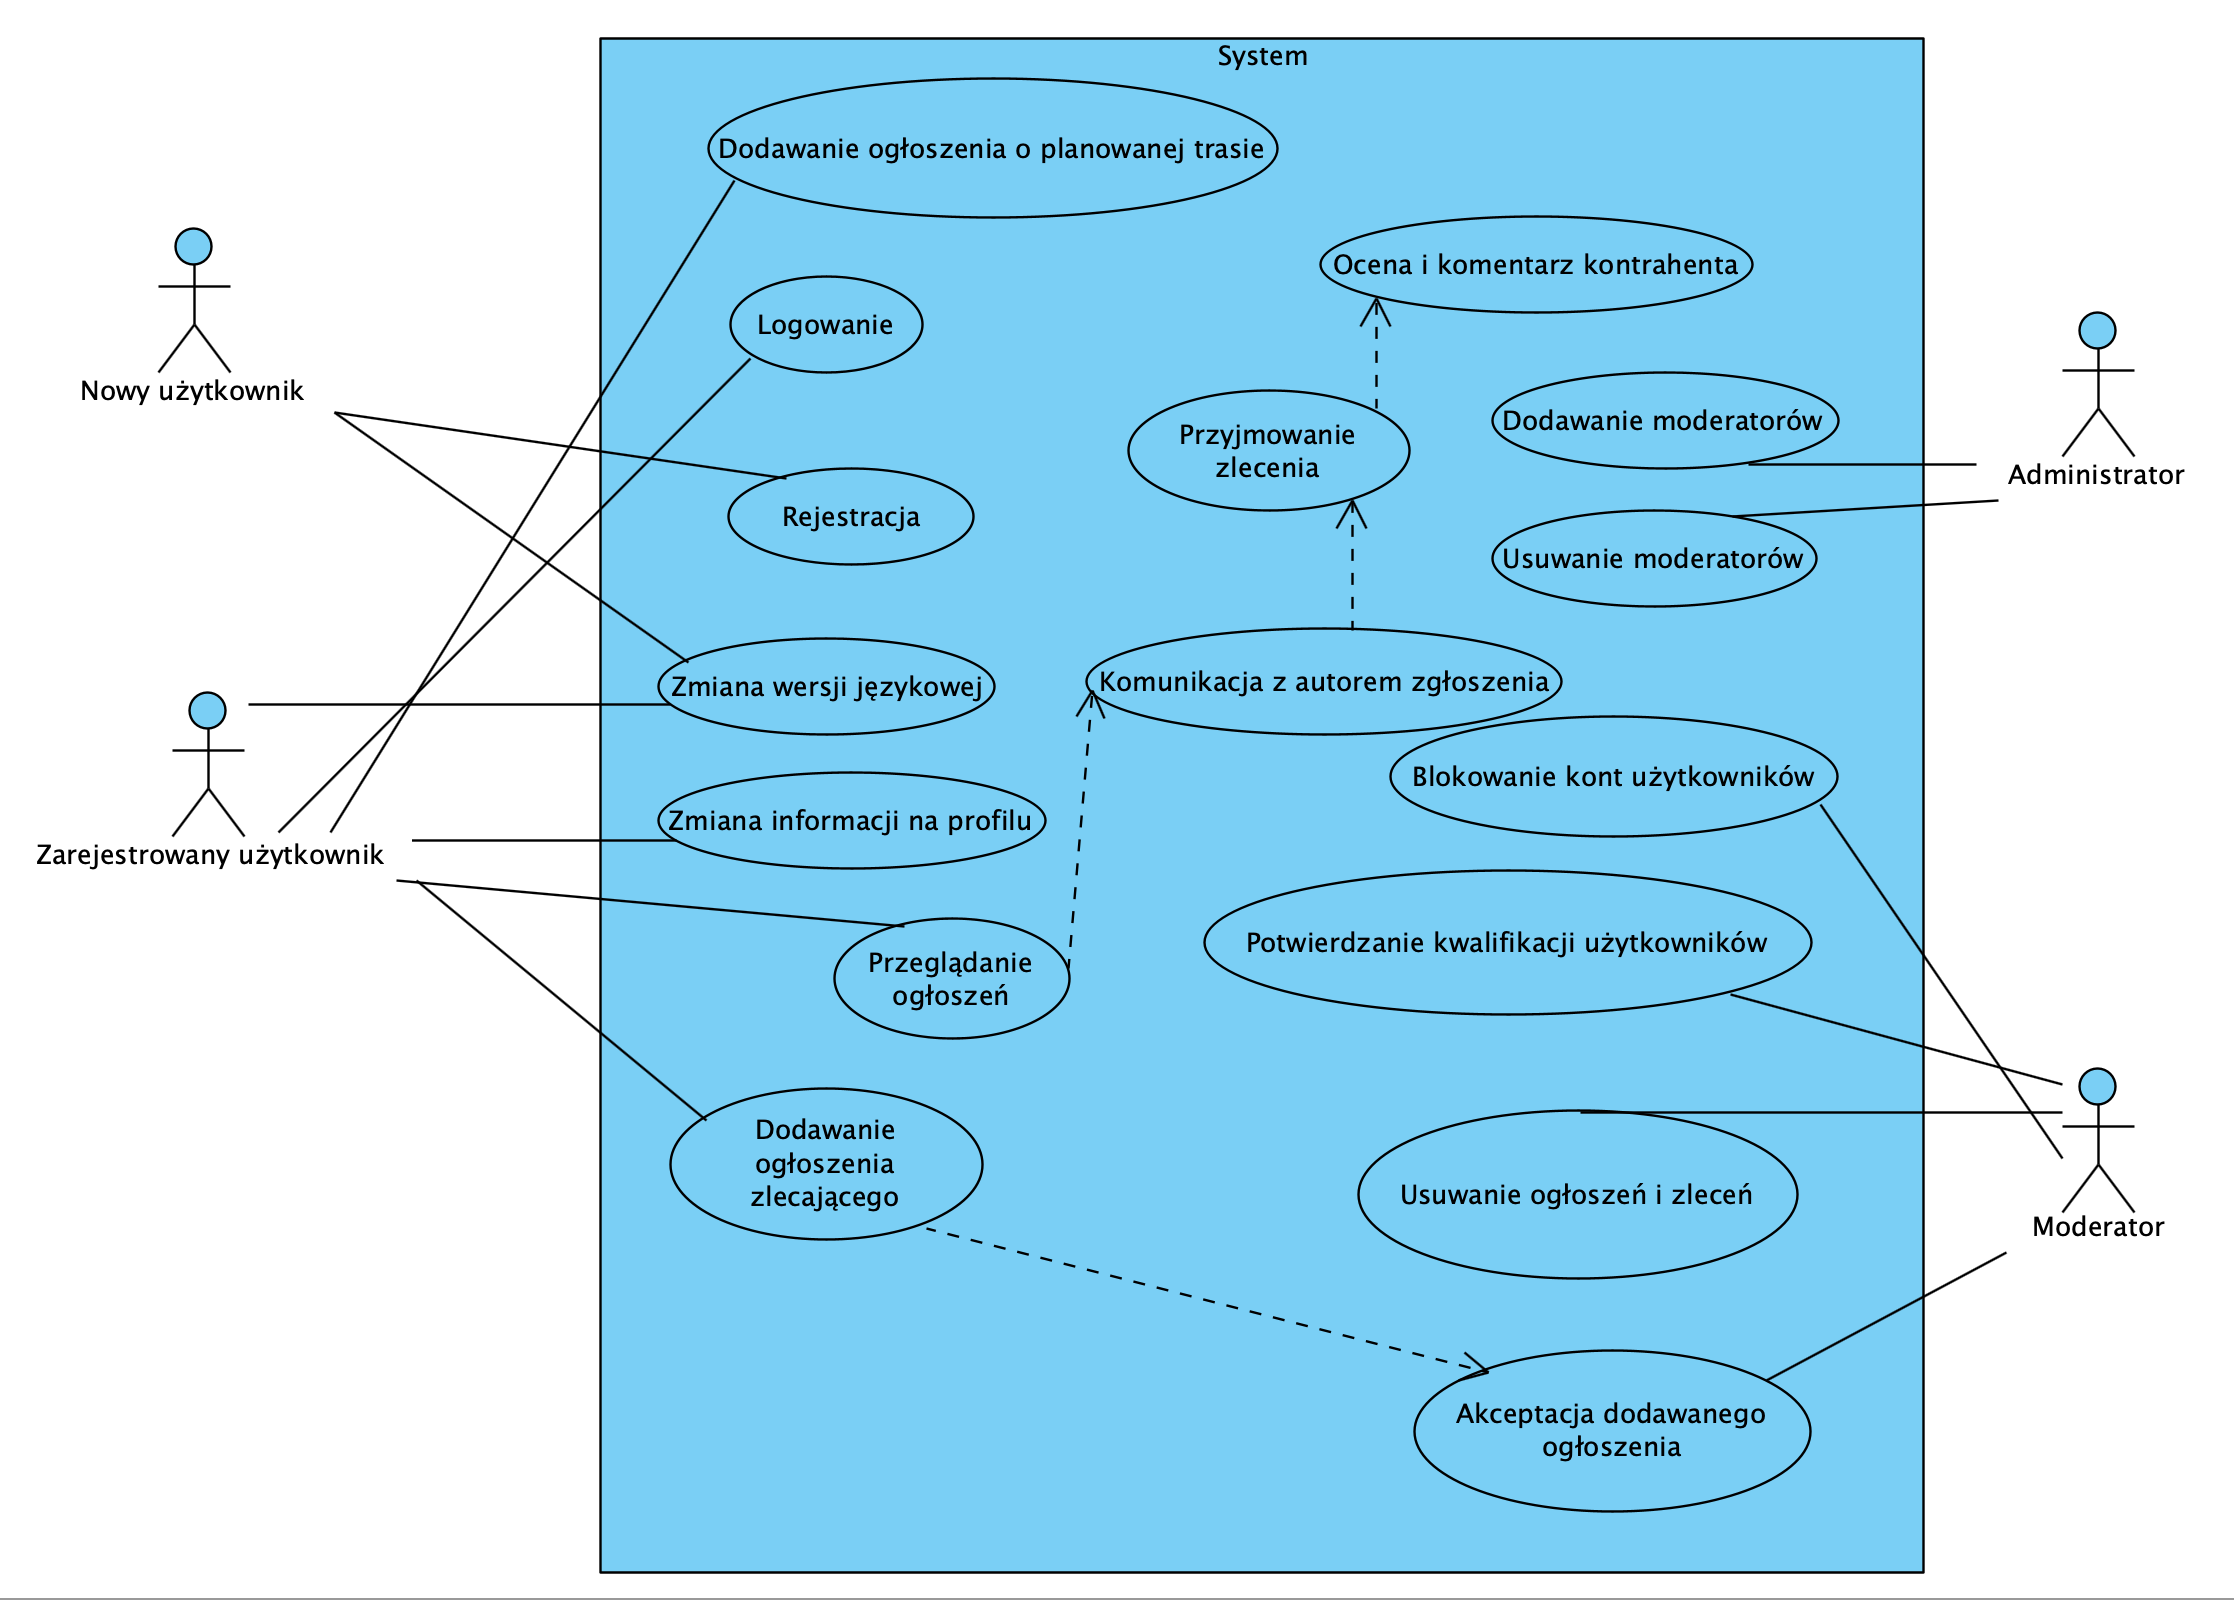
\includegraphics[width=0.9\linewidth]{rozdzial1/use_case.png}
	\caption{Przedstawienie przypadków użycia}
	\label{fig:Przedstawienie przypadków użycia}
\end{figure}

\chapter{Implementacja}
W niniejszym rozdziale przedstawiona zostanie szczegółowa analiza aspektów technicznych związanych z implementacją aplikacji. Na początku zaprezentowane zostaną wykorzystane narzędzia wraz z uzasadnieniem ich wyboru w kontekście wymagań projektowych. Następnie omówiona zostanie architektura warstw systemu. W dalszej części rozdziału szczegółowo opisane zostaną poszczególne moduły systemu oraz ich wzajemne powiązania. Następna część poświęcona będzie omówieniu implementacji kluczowych funkcjonalności: mechanizmu publikacji ogłoszeń, modułu wizualizacji tras na mapie oraz algorytmu rekomendacji ogłoszeń. W ostatniej części rozdziału przedstawione zostanie podejście do testowania aplikacji oraz proces jej wdrożenia na środowisko produkcyjne.

\section{Opis narzędzi}
Aplikacja została wykonana w technologii webowej, przy użyciu fullstackowego frameworka \texttt{Next.js} \cite{Next} (w wersji \texttt{15.1.3}). Jest to popularny sposób tworzenia aplikacji webowych, zapewniający wiele przydatnych funkcji poprawiających optymalizacje. Między innymi \texttt{Next.js} skraca czas potrzebny do załadowania aplikacji poprzez renderowanie kodu \texttt{HTML} strony, już podczas kompilacji aplikacji. Został on oparty na innym frameworku - React \cite{React}, jest to jedna z najpopularniejszych bibliotek \texttt{JavaScript} do budowania interfejsów użytkownika. Opiera się ona na koncepcji komponentów - niezależnych, wielokrotnego użytku bloków interfejsu. Komponenty te w  \texttt{Next.js} mogą być renderowane po stronie serwera, co znacząco przyspiesza pierwsze ładowanie strony. Dodatkowo renderowanie komponentów aplikacji po stronie serwera pozytywnie wpływa na algorytmy \texttt{SEO}, co skutkuje lepszym pozycjonowaniem serwisu w wyszukiwarkach internetowych. \texttt{Next.js} posiada zintegrowane rozwiązanie fullstackowe, oznacza to, że zarówno backend jak i frontend aplikacji wykorzystują tę samą bazę kodu. Takie podejście znacząco upraszcza proces developmentu i utrzymania aplikacji, eliminując potrzebę zarządzania oddzielnymi projektami dla części serwerowej i klienckiej. Dodatkowo ułatwia proces wdrożenia aplikacji na środowisko produkcyjne.

Zamiast standardowych klas \texttt{CSS}, do interfejsu użytkownika została użyta biblioteka \texttt{Tailwind} \cite{Tailwind} (w wersji \texttt{3.4.1}). Jest to narzędzie typu \texttt{utility-first CSS}, które pozwala na szybkie tworzenie responsywnych interfejsów poprzez zastosowanie predefiniowanych klas bezpośrednio w kodzie HTML.

Do wyświetlania na mapie tras z ogłoszeń użyte zostało \texttt{API Leaflet}. Jest to darmowy serwis oferujący interaktywne mapy, który umożliwia łatwą implementację funkcjonalności takich jak: wyświetlanie markerów, rysowanie tras czy obsługa zdarzeń związanych z interakcją użytkownika z mapą. Biblioteka została zoptymalizowana pod kątem urządzeń mobilnych, zapewniając płynne działanie i responsywność na różnych rozmiarach ekranów.

Testy jednostkowe aplikacji wykonane zostały przy użyciu biblioteki \texttt{Jest} \cite{Jest} (w wersji \texttt{29.7.0}). Framework ten został wybrany ze względu na jego natywną integrację z \texttt{Next.js} oraz możliwość łatwego tworzenia i uruchamiania testów dla komponentów React.

W celu usprawnienia procesu wdrożenia aplikacji na środowisko produkcyjne, zastosowano narzędzie \texttt{Docker} \cite{Docker}. Technologia ta pozwala na izolację poszczególnych modułów aplikacji w dedykowanych kontenerach, zapewniając jednakowe środowisko uruchomieniowe niezależnie od platformy. Kontenery \texttt{Docker} stanowią wyizolowane, lekkie maszyny wirtualne, w których uruchamiana jest aplikacja. Zastosowanie takiej architektury umożliwia zdefiniowanie wszystkich wymaganych zależności na etapie budowania obrazu kontenera, eliminując konieczność ich konfiguracji w środowisku produkcyjnym.

\section{Opis architektury}
TODO
\subsection{Architektura warstw}
\begin{figure}[H]
	\centering
		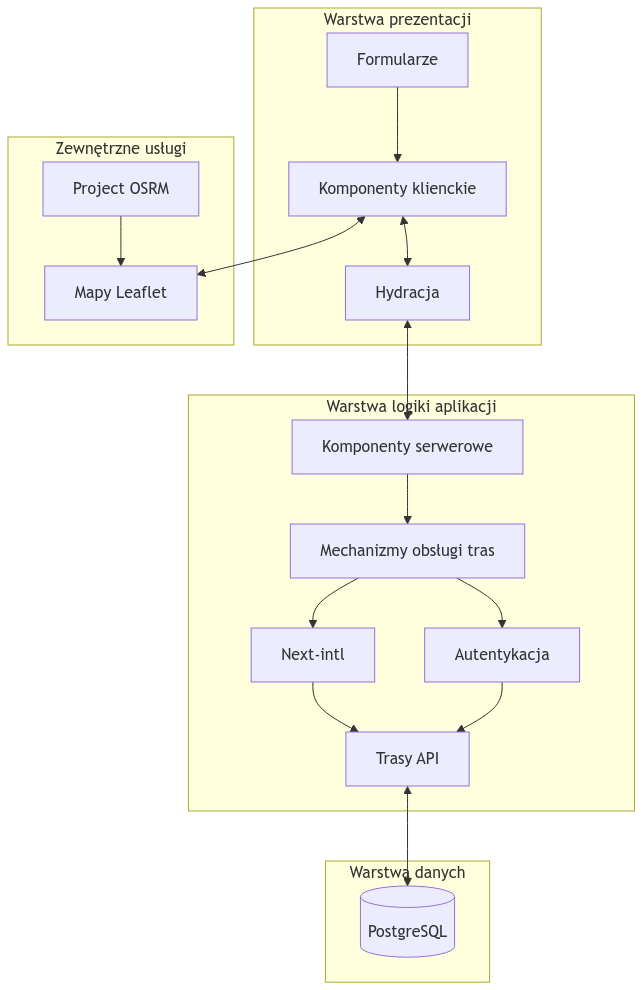
\includegraphics[width=0.7\linewidth]{rozdzial2/diagram_warstw.png}
	\caption{Diagram architektury warstw aplikacji}
	\label{Diagram warstw}
\end{figure}
Powyższy diagram przedstawia architekture warstw aplikacji. Zostały na nim wyszczególnione następujące warstwy:
\begin{enumerate}
    \item \textbf{Warstwa prezentacji} - odpowiada za bezpośrednią interakcje z użytkownikiem. W jej skład wchodzą:
    \begin{enumerate}
        \item Formularze - stanowią pośrednika między użytkownikiem, a warstwą logiki aplikacji. Pozwalają na wysyłanie wprowadzonych danych do warstwy logiki aplikacji,
        \item Komponenty klienckie (ang. \emph{client components}) - interaktywne elementy interfejsu użytkownika renderowane po stronie przeglądarki końcowego użytkownika, które:
        \begin{itemize}
            \item obsługują zdarzenia użytkownika (kliknięcia, wprowadzanie danych),
            \item zarządzają stanem lokalnym aplikacji przy użyciu haków React (ang. \emph{React hooks}),
            \item implementują dynamiczne zachowania interfejsu bez przeładowywania strony,
            \item komunikują się z API poprzez żądania HTTP,
            \item renderują interaktywne elementy mapy przy użyciu biblioteki Leaflet.
        \end{itemize}
        \item Hydracja - kluczowy proces w architekturze aplikacji \texttt{Next.js}. Przekształca początkowy, statyczny widok strony w pełni interaktywną aplikację React. Poprzez wypełnianie komponentów klienckich danymi pozyskanymi z warstwy logicznej aplikacji.
    \end{enumerate}
    \item \textbf{Warstwa logiki aplikacji} - są w niej zawarte wszelkie mechanizmy, do których użytkownik końcowy nie może mieć wglądu z uwagi na bezpieczeństwo. Warstwa ta składa się z:
    \begin{enumerate}
        \item Komponentów serwerowych (ang. \emph{server components}) - komponenty intefejsu użytkownika, które:
        \begin{itemize}
            \item są renderowane po stronie serwera, a użytkownikowi zwracany jest gotowy kod HTML,
            \item redukują ilość JavaScript przesyłanego do przeglądarki,
            \item mogą bezpośrednio komunikować się z bazą danych,
            \item mają dostęp do wrażliwych danych i zmiennych środowiskowych,
            \item są odpowiednie do renderowania statycznej zawartości i elementów niewymagających interaktywności.
        \end{itemize}
        \item Mechanizmów obsługi tras (ang. \emph{route handlers}) - odpowiadają za przetwarzanie żądań przychodzących i wysyłanie odpowiedzi.
        \begin{itemize}
            \item obsługują metody HTTP (\emph{GET, POST, PUT, DELETE}),
            \item zapewniają bezpieczną komunikację między frontendem a backendem aplikacji.
        \end{itemize}
        \item Next-intl - biblioteka do internalizacji, jest ona wykorzystywana do prezentacji treści w różnych językach (polskim, angielskim oraz niemieckim).
        \item Autentykacja - zapewnia bezpieczeństwo poprzez blokowanie wybranych tras API nieautoryzowanym użytkownikom.
        \item Trasy API - specjalne endpointy w aplikacji, są wykorzystywane do:
        \begin{itemize}
            \item zarządzania ogłoszeniami (dodawanie, zatwierdzanie, usuwanie zleceń),
            \item obsługi procesu rejestracji i logowania użytkowników,
            \item pobierania i filtrowania listy dostępnych ogłoszeń,
            \item komunikacji z zewnętrznym API OSRM dla wyznaczania tras,
        \end{itemize}
    \end{enumerate}
    \item \textbf{Warstwa danych} - Warstwa odpowiadająca za przechowywanie oraz dostarczanie wszelkich danych aplikacji. W aplikacji wykorzystano relacyjną bazę danych PostgreSQL, która przechowuje informacje o:
    \begin{itemize}
        \item użytkownikach systemu i ich rolach,
        \item zleceniach transportowych i ich statusach,
        \item lokalizacjach geograficznych (punkty początkowe i końcowe tras),
        \item czatach między użytkownikami oraz umowami zawartymi między nimi,
    \end{itemize}
    \item \textbf{Zewnętrzne usługi} - systemy i API wykorzystywane do rozszerzenia funkcjonalności aplikacji:
    \begin{enumerate}
        \item Project OSRM (ang. \emph{Open Source Routing Machine}), używany jest do zapewnia funkcji wyznaczania tras między punktami. Oferuje API do integracji z aplikacjami transportowymi.
        \item Mapy Leaflet, jest to biblioteka służąca do interaktywnej wizualizacji map, która umożliwia wyświetlanie markerów lokalizacji. Pozwala również na rysowanie tras na mapie oraz zapewnia intuicyjną nawigację i przybliżanie mapy.
    \end{enumerate}
\end{enumerate}

\section{Opis implementacji}
TODO

\subsection{Implementacja mechanizmu publikacji ogłoszeń o planowanej trasie}
\label{addAnnouncement}
Dodawanie nowego ogłoszenia o planowanej trasie odbywa się poprzez wysłanie przez użytkownika wypełnienionego formularza. W bazie danych muszą zostać zawarte informacje o: adresie początkowym, adresie końcowym, datach odjazdu i przyjazdu, tytule ogłoszenia oraz jego opisie, a także o ładowności pojazdu (maksymalny ciężar towaru, maksymalne wymiary towaru oraz maksymalna wysokość towaru). Walidacja wprowadzonych przez użytkownika danych odbywa się po stronie serwera. Poniżej zamieszczony został fragment funkcji dodającej do bazy danych nowe ogłoszenie o planowanej trasie.

{\belowcaptionskip=-9pt
\begin{lstlisting}[language=JavaScript,caption=Wstępna walidacja danych przed dodaniem ogłoszenia do bazy danych, label=lst:addAnnouncement]
export async function addAnnouncement(state: NewAnnouncementFormState, formData: FormData) {
  const t = await getTranslations('addPost');
  const validatedFields = newAnnouncementSchema(t).safeParse({
    title: formData.get('title'),
    brand: formData.get('brand'),
    model: formData.get('model'),
    maxWeight: formData.get('maxWeight'),
    maxSize: formData.get('maxSize'),
    maxHeight: formData.get('maxHeight'),
    fromCity: formData.get('fromCity'),
    toCity: formData.get('toCity'),
    departureDate: formData.get('departureDate'),
    arrivalDate: formData.get('arrivalDate'),
    desc: formData.get('desc'),
    from: JSON.parse(formData.get('from') as string) as Address,
    to: JSON.parse(formData.get('to') as string) as Address,
  });
  if (!validatedFields.success) {
    return {
      errors: validatedFields.error.flatten().fieldErrors,
    };
  }
  // Dalszy fragment funkcji
}
\end{lstlisting}
}

W powyższym fragmencie funkcji \texttt{addAnnouncement} widoczny jest mechanizm dodawania nowego ogłoszenia o planowanej trasie. Funkcja realizuje kilka kluczowych zadań:
\begin{enumerate}
    \item \textbf{Walidacja danych wejściowych} - funkcja wykorzystuje schemat walidacji \texttt{newAnnouncementSchema} zdefiniowany przy pomocy biblioteki \texttt{Zod}. Do schematu podawana jako argument jest funkcja pobierająca tłumaczenia dla komunikatów błędów.
    \item \textbf{Obsługa danych} - dane są pobierane z obiektu \texttt{FormData}, dostarczanego podczas wysyłania formularza. Adresy początkowy i końcowy są parsowane z objektu \texttt{JSON} zawierającego dokładne informacje o: współrzędnych, identyfikatorów krajów, stanów, miast, kodzie pocztowym oraz innych niezbędnych danych.
    \item \textbf{Mechanizm obsługi błędów} - w przypadku niepowodzenia walidacji funkcja zwraca do formularza obiekt z wyszczególnionymi błędami dla poszczególnych pól.
\end{enumerate}

Walidacja danych odbywa się po stronie serwera, jest to bezpieczniejszy sposób niż walidacja po stronie klienta, gdyż użytkownik końcowy nie ma wglądu w kod sprawdzający poprawność danych i nie może go obejść.

{\belowcaptionskip=-9pt
\begin{lstlisting}[language=JavaScript,caption=Schemat walidacji danych wejściowych, label=lst:addAnnouncementSchema]
export const newAnnouncementSchema = (t: any) =>
  z.object({
    title: z
      .string()
      .min(1, { message: t('mustNotBeEmpty') })
      .trim(),
    brand: z
      .string()
      .min(1, { message: t('mustNotBeEmpty') })
      .trim(),
    model: z
      .string()
      .min(1, { message: t('mustNotBeEmpty') })
      .trim(),
    maxWeight: z.coerce
      .number()
      .refine(inRange(1,50000), { message: t('valueBetween') + '1-50000' }),
    maxSize: z.string().regex(/^[1-9][0-9]*x[1-9][0-9]*$/, {
      message: t('formatIssue'),
    }),
    maxHeight: z.coerce
      .number()
      .refine(inRange(1, 1000), { message: t('valueBetween') + '1-1000' }),
    desc: z.string().trim(),
    departureDate: z.coerce.date(),
    arrivalDate: z.coerce.date(),
    from: AddressSchema(t),
    to: AddressSchema(t),
  });
\end{lstlisting}
}

Przedstawiony schemat walidacji danych wejściowych \texttt{newAnnouncementSchema} definiuje reguły sprawdzania poprawności dla nowego ogłoszenia transportowego przy użyciu biblioteki Zod. Schemat obejmuje następujące kluczowe elementy:
\begin{enumerate}
    \item \textbf{Walidacja tekstowa} - pola takie jak tytuł, marka, model wymagają niepustej wartości, która jest dodatkowo przycinana z białych znaków.
    \item \textbf{Walidacja liczbowa} - maksymalna waga towaru musi zawierać w zakresie 1-50000, a maksymalna wysokość towaru w zakresie 1-1000.
    \item \textbf{Walidacja formatu} - maksymalny rozmiar towaru wymaga formatu \emph{szerokość} x \emph{wysokość} liczonych w europaletach (np. 3x2). Daty wyjazdu i przyjazdu są konwertowane do formatu daty.
    \item \textbf{Walidacja adresów} - wykorzystuje osobny schemat \texttt{AddressSchema} dla weryfikacji danych adresowych.
\end{enumerate}
Schemat używa funkcji tłumaczącej do generowania komunikatów błędów, co zapewnia internacjonalizację komunikatów walidacyjnych.

Jeżeli wprowadzone dane zostaną pozytywnie rozpatrzone przez walidacje, następuje dodanie ogłoszenia o planowanej trasie do bazy danych.

{\belowcaptionskip=-9pt
\begin{lstlisting}[language=JavaScript,caption=Implementacja dodawania ogłoszenia do bazy danych, label=lst:addAnnouncementToDB]

export async function addAnnouncement(state: NewAnnouncementFormState, formData: FormData) {
    
    // Powyzej opisana walidacja danych

    const data = validatedFields.data;
    let [size_x, size_y] = data.maxSize.split('x').map(Number);
    const { userId } = await verifySession();
    
    const from_address_id = await addAddress(data.from);
    const to_address_id = await addAddress(data.to);
    
    await sql(
        'INSERT INTO announcements (title,description,start_date,arrive_date,max_weight,size_x,size_y,max_height,author_id,is_accepted,vehicle_brand,vehicle_model,from_address_id,to_address_id,road_color)VALUES($1,$2,$3,$4,$5,$6,$7,$8,$9,$10,$11,$12,$13,$14,$15)',
        [
        data.title,
        data.desc,
        data.departureDate,
        data.arrivalDate,
        data.maxWeight,
        size_x,
        size_y,
        data.maxHeight,
        userId,
        false,
        data.brand,
        data.model,
        from_address_id,
        to_address_id,
        '#' + ((Math.random() * 0xffffff) << 0).toString(16),
        ],
    );
    redirect({ locale: 'pl', href: '/announcements' });
}
\end{lstlisting}
}

\pagebreak
Powyższy fragment funkcji \texttt{addAnnouncement} realizuje proces zapisu nowego ogłoszenia transportowego do bazy danych. Wykonwane są w nim następujące czynności:
\begin{enumerate}
    \item \textbf{Przygotowanie danych} - parsuje rozmiar towaru na osobne wartości \texttt{size\_x} i \texttt{size\_y}, a także weryfikuje czy użytkownik w rzeczywiście jest zalogowany. Następnie do tabeli \texttt{addresses} dodawane są rekordy z adresem początkowym oraz końcowym.
    \item \textbf{Zapis do bazy danych} - dodaje rekord do tabeli \texttt{announcements} używając wszystkich przesłanych przez użytkownika danych. Odbywa się to poprzez używanie zmiennych (\$1, \$2, ...), uodparnia to aplikacje na atak typu \texttt{SQL injection}.
    \item \textbf{Automatyczne przekierowanie do listy ogłoszeń po pomyślnym dodaniu}.
\end{enumerate}
Domyślnie kolumna \texttt{is\_accepted} jest ustawiona na \texttt{false} ze względu na to, że ogłoszenie nie powinno być było widoczne publicznie natychmiast po dodaniu. Stanie się ono widoczne dopiero kiedy jeden z moderatorów je zatwierdzi. Wartość kolumny \texttt{road\_color} jest generowana losowo, kolor ten będzie używany do rysowania trasy przewozu na mapie.

\subsection{Implementacja wizualizacji tras na mapie}
W aplikacji użyto darmową open-source'ową biblioteke Leaflet, pozwala ona na wygenerowanie interaktywnej mapy, na której wyświetlane będą punkty oraz trasy. Wyświetlenie rzeczywistej trasy między punktami wymaga posiadania bazy danych ze współrzędnymi geograficznym wszystkich dróg na świecie. W aplikacji posłużono się gotowym darmowym rozwiązaniem w formie API. \texttt{Project OSRM} (ang. \emph{Open Source Routing Machine}) pozwala na wygenerowanie macierzy współrzędnych geograficznych, wskazujących na najkrótszą drogę między dwoma punktami.

{\belowcaptionskip=-9pt
\begin{lstlisting}[language=JavaScript,caption=Argumenty komponentu mapy, label=lst:mapProps]

export type Road = {
  from?: GeoPoint;
  to?: GeoPoint;
  postId?: string;
  color?: string;
};

type MapProps = {
  zoom?: number;
  className?: string;
  roads?: Road[];
};

export default function Map({ zoom = 13, className, roads = [] }: MapProps) {
// Dalszy fragment komponentu mapy
}
\end{lstlisting}
}

Komponent \texttt{Map} przyjmuje w argumencie wartość \texttt{zoom}, czyli poziom przybliżenia mapy, domyślnie w aplikacji ta wartość została ustawiona na 13, co daje nam widok na całą Europę. Argument \texttt{className} to klasy Tailwind, pozwala na stylizacje komponentu w zależności od potrzeb. Ostatni argument \texttt{roads} to tablica typu \texttt{Road}, typ ten zawiera informacje o trasie, współrzędnych geograficznych punktu początkowego oraz końcowego, identyfikator powiązanego z nią ogłoszenia oraz kolor rysowanej na mapie trasy.

\pagebreak
{\belowcaptionskip=-9pt
\begin{lstlisting}[language=JavaScript,caption=Implementacja pobierania najkrótszych tras między punktami, label=lst:fetchRoutes]
export default function Map({ zoom = 13, className, roads = [] }: MapProps) {
    
    const [routesPoints, setRoutesPoints] = useState<[number, number][][]>([]);
    const [selectedRoute, setSelectedRoute] = useState<number | null>(null);
    const t = useTranslations('map');

    useEffect(() => {
        const fetchRoutes = async () => {
        const newRoutes: [number, number][][] = [];
    
        for (const road of roads) {
            if (!road.from?.coordinates || !road.to?.coordinates) continue;
    
            try {
            const response = await fetch(
                `https://router.project-osrm.org/route/v1/driving/${road.from.coordinates[1]},${road.from.coordinates[0]};${road.to.coordinates[1]},${road.to.coordinates[0]}?overview=full&geometries=geojson`,
            );
    
            const data = await response.json();
    
            if (data.routes?.[0]?.geometry?.coordinates) {
                const points = data.routes[0].geometry.coordinates.map(
                (coord: [number, number]) => [coord[1], coord[0]] as [number, number],
                );
                newRoutes.push(points);
            }
            } catch (error) {
            console.error('Blad podczas pobierania trasy:', error);
            newRoutes.push([]);
            }
        }
    
        setRoutesPoints(newRoutes);
        };
    
        fetchRoutes();
    }, [roads]);
}
  \end{lstlisting}
}
  \pagebreak
  Powyższy fragment kodu ukazuje implementacje pobierania danych o najkrótszej trasie z API OSRM. Hak Reacta (ang. \emph{React Hook}) o nazwie \texttt{useEffect()} powoduje, że kod zawarty w tym haku, wykona się już po załadowaniu komponentu na stronie. Fragment ten spełnia następujące funkcje:
  \begin{enumerate}
    \item \textbf{Sprawdzanie poprawności argumentów} - zanim API OSRM zacznie być odpytywane, argument \texttt{roads} sprawdzany jest pod kątem posiadania w sobie pola ze współrzędnymi geograficznymi.
    \item \textbf{Wysyłanie zapytania do API OSRM} - zapytanie używa metody \texttt{GET} i są w nim zawarte informacje dotyczące współrzędnych geograficznych punktu początkowego oraz końcowego. Zauważyć można, że współrzędne podane są w odwrotny sposób niż ogólna przyjęta konwencja (najpierw szerokość, później długość), są to wymagania tego API.
    \item \textbf{Zamiana szerokości geograficznej z długością} - oprócz tego, że wymagane jest podawanie współrzędnych w odwróconej formie, to są one również w takiej formie zwracane. Po uzyskaniu odpowiedzi od API należy ją odwrócić.
    \item \textbf{Obsługa błędów} - jeżeli odpowiedź nie zostanie uzyskana lub zapytanie zwróci błąd, wówczas do konsoli aplikacji wypisywany jest komunikat o niepowodzeniu.
    \item \textbf{Ustawienie tras w stanie komponentu} - uzyskane macierze ze współrzędnymi geograficznymi tras, są ustawiane jako aktualny stan komponentu.
  \end{enumerate}
  
{\belowcaptionskip=-9pt
  \begin{lstlisting}[language=JavaScript,caption=Implementacja rysowania tras na mapie, label=lst:drawRoutes]
  export default function Map({ zoom = 13, className, roads = [] }: MapProps) {
  // Fragment kodu opisany powyzej
  return (
    <MapContainer
      center={roads[0]?.from?.coordinates ? [Number(roads[0].from.coordinates[0]), Number(roads[0].from.coordinates[1])] : undefined}
      zoom={zoom}
      scrollWheelZoom={true}
      className={`${className} z-10 h-screen w-full`}
    >
      
      {routesPoints.map(
        (points, index) =>
          points &&
          points.length > 0 && (
            <div key={index}>
              <Polyline
                key={index}
                positions={points}
                color={roads[index].color}
                weight={3}
                opacity={0.5}
                eventHandlers={{
                  click: () => {
                    setSelectedRoute(index);
                  },
                }}
              />
              {selectedRoute === index && (
                <Popup
                  position={points[Math.floor(points.length / 2)]}
                  eventHandlers={{
                    remove: () => setSelectedRoute(null),
                  }}
                >
                  <div>
                    <Link href={`/announcements/${roads[index].postId}`}>
                      Przejdz do ogloszenia
                    </Link>
                  </div>
                </Popup>
              )}
            </div>
          ),
      )}
    </MapContainer>
  );
}
\end{lstlisting}
}
Na powyższym fragmencie kodu zauważyć można renderowanie komponentu mapy z wykorzystaniem biblioteki Leaflet. Implementacja łączy pobrane wcześniej dane tras z interaktywną wizualizacją na mapie, umożliwiając użytkownikowi przeglądanie i eksplorację tras transportowych. Powyższy kod obejmuje następujące kluczowe funkcjonalności:
\begin{enumerate}
    \item \textbf{Inicjalizacja kontenera mapy} - ustawienie centrum mapy na podstawie współrzędnych pierwszej trasy, dodanie możliwości przewijania mapy za pomocą rolki myszy.
    \item \textbf{Renderowanie tras} - mapowanie pobranych wcześniej punktów tras. Rysowanie linii tras (\texttt{Polyline}) z indywidualnym kolorem dla każdej trasy.
    \item \textbf{Obsługa interakcji} - zaznaczanie wybranej trasy, wyświetlanie wyskakującego okna (ang. \emph{Popup}) po kliknięciu trasy. W oknie znajduję się odnośnik do powiązanego ogłoszenia.
\end{enumerate}
Połączenie powyższych fragmentów kodu pozwala na wyświetlenie interaktywnej mapy z trasami transportowymi, co stanowi kluczową funkcjonalność aplikacji.

\subsection{Implementacja algorytmu rekomendacji ogłoszeń}

Rekomendowanie ogłoszenia odbywa się w funkcji \texttt{addAnnouncement} \ref{addAnnouncement} jeszcze przed dodaniem ogłoszenia do bazy danych. Algorytm rekomendacji polega na znalezieniu ogłoszeń, które są najbardziej zbliżone do dodawanego ogłoszenia. W tym celu wykorzystywane są współrzędne geograficzne punktu początkowego i końcowego dodawanego ogłoszenia. Następnie obliczana jest odległość od punktów początkowych i końcowych innych ogłoszeń. Ogłoszenie, które wykaże odległość od punktu początkowego i punktu końcowego nie wiekszą niż 50km oraz zawiera się w odpowiednim zakresie właściwości fizycznych towaru, jest zwracane jako rekomendacja.

{\belowcaptionskip=-9pt 
\begin{lstlisting}[language=JavaScript,caption=Implementacja rekomendacji ogłoszeń, label=lst:recomendPost]
  export async function tryLinkToPost(post: ErrandProps | AnnouncementProps): Promise<string | null> {
  if ('ware' in post) {
    const announcements = await getAnnouncements(SortDirection.ByNewest);
    const match = announcements.find((announcement) =>
      isMatchingDelivery(
        post.from.geography!,
        announcement.from.geography!,
        post.to.geography!,
        announcement.to.geography!,
        post.ware,
        announcement.carProps,
      ),
    );
    return match?.id ?? null;
  } else {
    const errands = await getErrands(SortDirection.ByNewest);
    const match = errands.find((errand) =>
      isMatchingDelivery(
        post.from.geography!,
        errand.from.geography!,
        post.to.geography!,
        errand.to.geography!,
        errand.ware,
        post.carProps,
      ),
    );
    return match?.id ?? null;
  }
}
\end{lstlisting}
}

Powyższy fragment kodu przedstawia implementację algorytmu rekomendacji ogłoszeń. Funkcja \texttt{tryLinkToPost} przyjmuje jako argument ogłoszenie, które ma zostać zarekomendowane. W zależności od tego czy ogłoszenie jest ogłoszeniem o planowanej trasie czy zleceniem transportowym, pobierane są odpowiednie ogłoszenia z bazy danych. Następnie dla każdego ogłoszenia sprawdzane jest czy spełnia ono warunki rekomendacji.

{\belowcaptionskip=-9pt
\begin{lstlisting}[language=JavaScript,caption=Funkcja sprawdzająca warunki powiązania ogłoszeń, label=lst:isMatchingDelivery]
    export function isMatchingDelivery (
    fromPoint1: GeoPoint,
    fromPoint2: GeoPoint,
    toPoint1: GeoPoint,
    toPoint2: GeoPoint,
    ware: ErrandProps['ware'],
    carProps: AnnouncementProps['carProps']
  ): boolean {
    const isStartPointValid = arePointsInRange(fromPoint1, fromPoint2, 50);
    const isEndPointValid = arePointsInRange(toPoint1, toPoint2, 50);
    const areSizesValid = areDimensionsValid(ware, carProps);

    return isStartPointValid && isEndPointValid && areSizesValid;
  }
\end{lstlisting}
}

Funkcja \texttt{isMatchingDelivery} sprawdza czy dane ogłoszenie spełnia warunki rekomendacji. W zależności od tego czy punkty początkowe i końcowe ogłoszeń znajdują się w odpowiedniej odległości od siebie oraz czy wymiary towaru mieszczą się w zakresie wymiarów pojazdu, funkcja zwraca wartość \texttt{true} lub \texttt{false}.

{\belowcaptionskip=-9pt
\begin{lstlisting}[language=JavaScript,caption=Funkcje obliczająca odległość między punktami, label=lst:calculateDistance]
  export function calculateDistance(point1: GeoPoint, point2: GeoPoint): number {
    const R = 6371;
  
    const lat1 = (parseFloat(point1.coordinates[0]) * Math.PI) / 180;
    const lon1 = (parseFloat(point1.coordinates[1]) * Math.PI) / 180;
    const lat2 = (parseFloat(point2.coordinates[0]) * Math.PI) / 180;
    const lon2 = (parseFloat(point2.coordinates[1]) * Math.PI) / 180;
  
    const dLat = lat2 - lat1;
    const dLon = lon2 - lon1;
  
    const a =
      Math.sin(dLat / 2) * Math.sin(dLat / 2) +
      Math.cos(lat1) * Math.cos(lat2) * Math.sin(dLon / 2) * Math.sin(dLon / 2);
  
    const c = 2 * Math.atan2(Math.sqrt(a), Math.sqrt(1 - a));
    const distance = R * c;
  
    return Number(distance.toFixed(2));
  }
  
  export function arePointsInRange(point1: GeoPoint, point2: GeoPoint, maxDistance: number): boolean {
    return calculateDistance(point1, point2) <= maxDistance;
  }
\end{lstlisting}
}

W powyższym fragmencie kodu znajdują się funkcje pomocnicze wykorzystywane w algorytmie rekomendacji ogłoszeń. Funkcja \texttt{calculateDistance} oblicza odległość między dwoma punktami geograficznymi. Funkcja \texttt{arePointsInRange} sprawdza czy odległość między dwoma punktami nie przekracza maksymalnej odległości. Funkcja \texttt{areDimensionsValid} sprawdza czy wymiary towaru mieszczą się w wymiarach pojazdu. 

Do obliczenia odległości między punktami wykorzystany został wzór Haversine'a \cite{HeavenlyMathematics}. Wzór ten jest matematyczną metodą obliczania odległości między dwoma punktami na sferze (w tym przypadku na kuli ziemskiej) przy użyciu ich współrzędnych geograficznych (szerokości i długości). Jest on powrzechnie używany w nawigacji GPS oraz w systemach geolokalizacyjnych. Wzór ten wymaga podania promienia sfery (dla Ziemi jest to 6371km), następnie przekształca stopnie na radiany oraz używa funkcji trygonometrycznych do obliczenia różnicy współrzędnych. Końcowy wynik jest zaokrąglany do dwóch miejsc po przecinku, co daje nam odległość liczoną w kilometrach.

\begin{equation}
  \text{dystans} = 2R \arcsin\left(\sqrt{\sin^2\left(\frac{\phi_2 - \phi_1}{2}\right) + \cos(\phi_1)\cos(\phi_2)\sin^2\left(\frac{\lambda_2 - \lambda_1}{2}\right)}\right)
\end{equation}

Gdzie: 
$R$ - promień Ziemi
$\phi_1, \phi_2$ - szerokości geograficzne
$\lambda_1, \lambda_2$ - długości geograficzne

{\belowcaptionskip=-9pt
\begin{lstlisting}[language=JavaScript,caption=Funkcja sprawdzająca czy ogłoszenie zawiera się w odpowiednim zakresie właściwości fizycznych towaru , label=lst:areDimensionValid]
export function areDimensionsValid(ware: ErrandProps['ware'], carProps: AnnouncementProps['carProps']): boolean {
  return (
    ware.weight <= carProps.maxWeight &&
    ware.size.height <= carProps.maxSize.height &&
    ware.size.x * ware.size.y <= carProps.maxSize.x * carProps.maxSize.y
  );
}
\end{lstlisting}
}

Funkcja \texttt{areDimensionsValid} sprawdza czy wymiary towaru mieszczą się w wymiarach pojazdu. Wartości te są porównywane z wartościami maksymalnymi pojazdu, jeżeli wszystkie wartości są mniejsze lub równe wartościom maksymalnym, to funkcja zwraca wartość \texttt{true}, w przeciwnym wypadku \texttt{false}.

\section{Opis testów aplikacji}
Aplikacja w trakcie implementacji była testowana na bieżąco. Testy obejmowały zarówno testy jednostkowe, integracyjne, jak i testy \texttt{end-to-end}. Testy jednostkowe sprawdzały poprawność działania poszczególnych komponentów, testy integracyjne sprawdzały poprawność współpracy poszczególnych komponentów aplikacji, a testy end-to-end sprawdzały poprawność działania aplikacji jako całości. Testy jednostkowe oraz integracyjne napisano w języku JavaScript przy użyciu biblioteki \texttt{Jest}, natomiast na potrzeby testów \texttt{end-to-end} użyte zostało narzędzie \texttt{Selenium IDE}.

\subsection{Testy jednostkowe}
Testy jednostkowe sprawdzają poprawność działania poszczególnych komponentów aplikacji. W aplikacji testowano następujące komponenty:
\begin{itemize}
  \item Pasek nawigacyjny, w kodzie aplikacji nazwany \texttt{Nav},
  \item Formularz rejestracji, w kodzie aplikacja nazwany \texttt{SignupForm},
  \item Wyświetlanie zlecenia, w kodzie aplikacji nazwany \texttt{Errand},
  \item Mapę z narysowanymi trasami, w kodzie aplikacji nazwany \texttt{AllRoadsMap},
\end{itemize}

Przykładowy test jednostkowy sprawdzający poprawność działania komponentu \texttt{Nav}, komponent ten został użyty międzyinnymi na stronie przeglądarki ogłoszeń o planowanych trasach \ref{Przeglądanie ogłoszeń planowanych tras}:

{\belowcaptionskip=-9pt
\begin{lstlisting}[language=JavaScript,caption=Przykładowy test jednostkowy paska nawigacyjnego, label=lst:NavTest]
it('opens mobile menu when hamburger icon is clicked', () => {
    render(
      <NextIntlClientProvider messages={messages} locale="pl">
        <Nav />
      </NextIntlClientProvider>,
    );

    const menuButton = screen.getByTestId('menu-button');
    fireEvent.click(menuButton);

    const sideMenu = screen.getByTestId('side-menu');
    const menuOverlay = screen.getByTestId('menu-overlay');

    expect(sideMenu).not.toHaveClass('hidden');
    expect(sideMenu).toHaveClass('fixed');
    expect(menuOverlay).toBeInTheDocument();
  });
\end{lstlisting}
}

Powyższy test sprawdza funkcjonalność otwierania menu mobilnego po kliknięciu w ikonę hamburgera. Sprawdza on czy, menu mobilne zostaje poprawnie otwarte, czy posiada odpowiednie klasy oraz czy overlay menu został wyrenderowany.

Inne testy jednostkowe dla tego komponentu sprawdzały poprawność nastepujących funkcjonalności:
\begin{enumerate}
  \item Renderowanie nagłówka z nazwą aplikacji.
  \item Czy mobilne menu jest domyślnie zamknięte.
  \item Czy menu mobilne jest poprawnie zamykane po kliknięciu ikony hamburgera.
  \item Czy nazwa obecnej strony jest poprawnie wyświetlana.
  \item Czy chowanie i pokazywanie menu nawigacji będzie poprawnie działać po kliknieciu dwukrotnie w ikonę hamburgera.
\end{enumerate}
\chapter{Podsumowanie i wnioski}

\section{Wykonane czynności}
W ramach pracy inżynierskiej opracowano projekt i implementację aplikacji webowej CargoLink, mającej na celu optymalizację procesów związanych z transportem towarów. Stworzona aplikacja umożliwia zleceniodawcom i przewoźnikom dodawanie ogłoszeń, dopasowywanie ofert, prowadzenie komunikacji oraz finalizowanie transakcji poprzez generowanie szablonów umów. System wprowadza także mechanizm ocen użytkowników, co wspiera budowanie zaufania między stronami.\\
W projekcie wykonano:
\begin{enumerate}
    \item \textbf{Analizę wymagań} - zidentyfikowano kluczowe potrzeby użytkowników i funkcjonalności systemu.
    \item \textbf{Projekt systemu} - opracowano diagramy przypadków użycia, projekt bazy danych oraz makiety interfejsu użytkownika z uwzględnieniem responsywności.
    \item \textbf{Implementację aplikacji} - wykorzystano technologie TypeScript, Next.js, Tailwind CSS i PostgreSQL. Zastosowano bezpieczne mechanizmy przechowywania danych, takie jak UUID dla identyfikatorów i bcrypt do szyfrowania haseł.
    \item \textbf{Testy} - przeprowadzono testy jednostkowe, end-to-end oraz wydajnościowe, zapewniając poprawność i stabilność działania systemu.
\end{enumerate}

\section{Napotkane problemy}

Początkowo projekt zakładał przechowywanie nazw miast początkowych i końcowych wraz ze współrzędnymi geograficznymi bezpośrednio w tabelach \texttt{announcements} i \texttt{errands}. Podczas implementacji odkryto jednak lukę: brakowało informacji o państwie i stanie lokalizacji.

Rozważano ręczne wprowadzanie tych danych przez użytkownika, ale mogłoby to negatywnie wpłynąć na wygodę korzystania z aplikacji. Alternatywą było utworzenie osobnej tabeli \texttt{addresses} przechowującej pełne informacje o adresach. Tym samym w tabelach \texttt{announcements} i \texttt{errands} pozostawiono jedynie klucze obce do tabeli \texttt{addresses}.

Zmiana wymusiła modyfikację formularzy dodawania ogłoszeń i zleceń - zamiast ręcznego wprowadzania, użytkownicy zyskali możliwość wyboru adresu z listy.

\section{Możliwości rozwoju}

Aplikacja została stworzona z myślą o rozwoju. W przyszłości można by dodać nowe funkcjonalności, takie jak:
\begin{itemize}
    \item Możliwość dodawania zdjęć do ogłoszeń i zleceń.
    \item Dodanie możliwości ingerencji w spór między użytkownikami.
    \item Rozbudowanie systemu oceniania użytkowników, możliwość oceniania dopiero po zakończeniu zlecenia.
    \item Zgłaszanie nieprawidłowości w ogłoszeniach i zleceniach.
    \item Dodanie możliwości wyboru dokładnej trasy przejazdu (jeżeli użytkownik nie chce korzystać z proponowanej trasy).
\end{itemize}

\section{Wnioski}

Projekt CargoLink stanowi innowacyjne rozwiązanie w obszarze transportu okazjonalnego, które przy wykorzystaniu nowoczesnych technologii (\texttt{TypeScript}, \texttt{Next.js}, \texttt{Tailwind CSS}, \texttt{Node.js}, \texttt{PostgreSQL}) oferuje kompleksową platformę łączącą przewoźników ze zleceniodawcami. Aplikacja przyczyni się do optymalizacji procesów logistycznych poprzez inteligentny system rekomendacji, bezpośrednią komunikację między użytkownikami, graficzną prezentację tras oraz wielojęzyczny interfejs, co pozwoli na redukcję kosztów transportu i eliminację nieefektywnego wykorzystania zasobów transportowych. Realizacja projektu stanowi odpowiedź na rosnące zapotrzebowanie rynku na narzędzia usprawniające współpracę w sektorze transportowym.

\bibliographystyle{plabbrv}
\setlength{\bibitemsep}{2pt}
\addtocontents{toc}{\addvspace{2pt}}
\bibliography{bibliografia}
\appendix

\chapter{Instrukcja wdrożeniowa}
Aplikacja jest konteneryzowana przy użyciu Docker, co zapewnia kompatybilność międzyplatformową. Baza danych jest hostowana na darmowym serwerze \texttt{Neon}, co upraszcza konfigurację.
\begin{itemize}
    \item Zainstalowane oprogramowanie \texttt{Docker}
    \item Dostęp do internetu
    \item Uprawnienia administratora
\end{itemize}
W celu wdrożenia aplikacji na środowisko produkcyjne należy wykonać następujące kroki:
\begin{enumerate}
    \item Sklonować repozytorium z GitHub.
    \item Otworzyć terminal w katalogu projektu.
    \item Zbudować obraz aplikacji za pomocą komendy \texttt{docker build -t cargolink .}.
    \item Uruchomić kontener z aplikacją za pomocą komendy \texttt{docker run -p 80:3000 cargolink}.
\end{enumerate}

Po wykonaniu powyższych kroków aplikacja będzie dostępna pod adresem \texttt{http://localhost:80}. Port na którym działa aplikacja można zmienić w pliku \texttt{Dockerfile} w linii 4. Jednak port 80 jest domyślnym portem dla protokołu HTTP, więc zaleca się pozostawienie go bez zmian. Jeżeli serwer, na którym wykonane zostały powyższe kroki, jest dostępny z zewnątrz, aplikacja będzie dostępna pod adresem \texttt{http://<adres\_serwera>:80}.

\end{document}
